\documentclass[de]{./../../common/SurferDesc}%%%%%%%%%%%%%%%%%%%%%%%%%%%%%%%%%%%%%%%%%%%%%%%%%%%%%%%%%%%%%%%%%%%%%%%
%
% The document starts here:
%
\begin{document}
\footnotesize
% Weltrekordfl�chen

%%% 1.Tafel

\begin{surferPage}
  \begin{surferTitle}Eine Septik mit 99 Singularit�ten\end{surferTitle}   \\
  
   Oliver Labs konstruierte im Rahmen seiner Dissertation in Mainz 2004 eine
    Fl�che vom Grad $7$ (Septik) mit $99$ Singularit�ten: derzeit Weltrekord! 
    Bisher ist aber kein Grund bekannt, warum es nicht sogar eine Septik mit
    $104$ Singulari�ten geben k�nnte!  
    Labs' Fl�che hat die Symmetrie eines regelm��igen $7$-Ecks.
    Man sieht dies recht gut, wenn man die Fl�che von ``oben'' betrachtet:
    \vspace*{-0.3em}
    \begin{center}
      \begin{tabular}{c@{\qquad}c}
        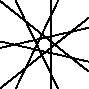
\includegraphics[height=1.5cm]{./../../common/images/labsseptic1.pdf}
        &
        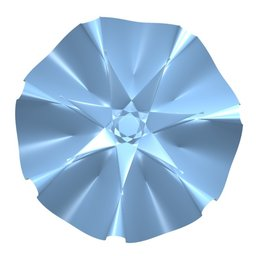
\includegraphics[height=1.5cm]{./../../common/images/labs_septic_von_oben}
      \end{tabular}
    \end{center}
    \vspace*{-0.3em}
    Zur Suche nach der Fl�che hat O.\ Labs das Computeralgebraprogramm
    {\sc Singular} (Universit\"at Kaiserslautern) benutzt, dessen besondere St�rke in
    Anwendungen auf 
    algebraischer Geometrie und Singularit�ten liegt.

    Dabei hat er ausgenutzt, dass man in endlichen
    Zahlensystemen rechnen kann. Von der Uhr kennen wir dies: 24 Uhr
    entspricht 0 Uhr, 24 Uhr $+$ 1 Stunde ist nicht 25 Uhr, sondern 1
    Uhr.      
\end{surferPage}


\end{document}
%
% end of the document.
%
%%%%%%%%%%%%%%%%%%%%%%%%%%%%%%%%%%%%%%%%%%%%%%%%%%%%%%%%%%%%%%%%%%%%%%%
